\documentclass[a4paper,11pt]{article}

%\usepackage[ngerman]{babel}
% use mac coding
%\usepackage[applemac]{inputenc}
%cite "`author ,year""
\usepackage{latexsym}
\usepackage{natbib,amsmath}
\usepackage{bm}
% neue Rechtschreibung, AMSMath, AMSSymb, A4 Format
\usepackage{amsmath,amssymb,a4wide}
%Grafiken, Zeilenabstand
\usepackage{graphicx, setspace}
%Bookmarks, Hyperlinks
\usepackage[bookmarks=true, bookmarksopen=true,
            bookmarksnumbered=true, colorlinks,citecolor = black,filecolor = black,
            linkcolor = black,urlcolor  = black,plainpages=false,hyperindex=true]{hyperref}
%index            
\usepackage{makeidx}
%pfad zu sweave package 
%\usepackage{/Library/Frameworks/R.framework/Resources/share/texmf/Sweave}      
% pdf einstellungen
\hypersetup{
       pdftitle={},
       pdfauthor={Robert Ferstl, Josef Hayden},
       pdfsubject={Inhalt},
        pdfkeywords={}
        pdfcreator={},
       pdfproducer={}
     }     
%Absatzabstaende
\setlength{\parindent}{0.0cm} \setlength{\parskip}{1.5ex plus
0.5ex minus 0.5ex}
%Zeilenabstand in Tabellen
\renewcommand{\arraystretch}{2}

%\pagestyle{headings} 

\usepackage{natbib}


\usepackage{listings}
\usepackage{color}











\title{termstrc: A Package for Term Structure Estimation with R}


\author{Robert Ferstl\hspace{0.5cm}Josef Hayden}


 %Index
\makeindex
           
\begin{document}

%define colors for syntax highlighting
\definecolor{darkblue}{rgb}{0,0,.5}
\definecolor{darkred}{rgb}{0.4,0.0,0}
\definecolor{commentcolor}{rgb}{0,0.5,0.25}
\definecolor{stringcolor}{rgb}{0.5,0.0,0}

%settings for R syntaxhighlighting
\lstset{basicstyle=\ttfamily\small,
keywordstyle=\bfseries\color{darkblue},
stringstyle=\ttfamily,
showstringspaces=false,
language=R,
identifierstyle=,
commentstyle=\color{commentcolor},
stringstyle=\color{stringcolor}}
  \maketitle
  
  \abstract{
Zero-coupon yield curves and credit spread curves are important inputs for various financial models, e.g. pricing of securities, risk management, monetary policy issues. Since zero-coupon rates are rarely directly observable, they have to be estimated from market data for existing coupon bonds. The literature broadly distinguishes between parametric and spline-based methods. We implement two widely-used term structure estimation procedures, i.e. the parametric Nelson and Siegel approach and the Svensson approach.
  
Moreover, we implement the traditional way of credit spread calculation, where individually estimated zero-coupon yield curves are substracted from a risk-free reference curve. Goodness-of-fit tests are provided to compare the results of the different estimation methods. We illustrate the usage of our functions by practical examples with data from European and CEE government bonds, and European corporate bonds.
}
  \section{Introduction}
 
 
The R package termstrc consist of methods for estimating the term structure of interest rates from market data. 
  
In this section we will provide the basic concepts which are required for the estimation of the term structure. Section 2 covers the two models behind our algorithm. An explaination in an formal notation of the used term structure estimation approach is presented in section 3. The examples in section 4 complement the theoretical framework and introduce the usage of the termstrc package. 


Since zero-coupon rates are rarely directly observable, they have to be estimated from market data for existing coupon bonds.
At the market the following characteristica of a bond $j$ are observable: the maturity date $m$ , the clean price $p_c$, the cashflow $c_t$ (coupon and redemption payments) which occurs at $t=1...n$.  An investor who wants to buy the bond $i$ has to pay the dirty price $p_d$ which consists of the quoted market price (clean price) $p_c$ and the accrued interest $a$.

The term structure of interest rates can usually be described in three ways: the discount function, the 
spot rate function and the forward rate function.  We will use the idea of the discount and spotrate function. Therefore we briefly explain the two concepts. 

The bond price equation for a bond $j$ under continuous compounding is the present value of all cashflows.


%duration

\begin{equation}
  \label{bondpriceeq}
  p_c+a = \sum_{t=1}^n \ c_t e^{-s_tm_t}
\end{equation}

The spot rate $s_t$ is the yield-to maturity for a $t$-period zero-coupon bond. $m_t$ is the time to maturity of the $t$-th cash flow. A plot of the yields against times to maturity produces the zero-coupon yield curve.

The yield-to-maturity is the solution for $y$ in the following equation.

\begin{equation}
  \label{yield}
  p_c+a=\sum_{t=1}^n \ c_t e^{-ym_t}
\end{equation}

An equivalent formulation of the bond price equation makes use of the discount factors $d_t=\delta(m_t)=e^{-s_tm_t}$. The continuous discount function $\delta(\cdot)$ is formed by interpolation of the discount factors. 

\begin{equation}
  \label{bondprceq2}
  p_c+a=\sum_{t=1}^n \ c_t \delta(m_t) \end{equation}
 

 
 \section{The Nelson/Siegel and Svensson method}

\label{nels-svenss-meth}
 Under the assumption that a function between the spot rates and maturities exists, the term structure can be estimated. 
 
\cite{Nelson1987} proposed a parsimonious model of the yield curve. They model the spote rate with a second order differential equation. 

\begin{equation}\label{ns_spot}
    s(m,\bm{b}) = \beta_0 + \beta_1\frac{1-\exp(-\frac{m}{\tau_1})}{\frac{m}{\tau_1}} + \beta_2\left(\frac{1-\exp(-\frac{m}{\tau_1})}{\frac{m}{\tau_1}} - \exp(-\frac{m}{\tau_1})\right)
\end{equation}

The choice of the parameters ${\bm{b}} = \left(\beta_0,\beta_1,\beta_2,\tau_1\right)$ enables us to construct various possible shapes of the spot rate and the instantenous  forward rate curve. The constant term $\beta_0$ is the limit of the  instantenous forward rate when the time to maturity tends to infinity. The first exponential term $\beta_1 \exp(-\frac{m}{\tau_1})$ can be interpreted as a short-term contribution. It will decrease monotonically to zero with time to maturity when $\beta_1$ is positive. The second exponential term $\beta_2 \frac{m}{\tau_1} \exp(-\frac{m}{\tau_1})$ generates a hump-shape, which is realized in the medium term, because it starts at zero and decays to zero. 

The following code replicates figure 2 on page 477 in \cite{Nelson1987}.

\begin{verbatim}
m <- seq(0,10,0.01)
beta_1 <- 1
tau_1 <- 1
beta_2 <- 1
beta_0 <- 1

par(lwd=2)
plot(m,beta_1*exp(-m/tau_1),type="l",col=1,
     xlab="Time to maturity",
     ylab="Model curves",ylim=c(0,2.1),lty=4)
     
lines(m,beta_2*(m/tau_1)*exp(-m/tau_1),lty=2,col=2)

lines(m,beta_0+beta_1*exp(-m/tau_1)+beta_2*(m/tau_1)*exp(-m/tau_1),col=3)

abline(h=1,lty=3,col=4)

legend("topright",legend=c(expression(beta[1]*exp(-m/tau[1])), 
       expression(beta[2]*(m/tau[1])*exp(-m/tau[1])),
       expression(beta[0]),
       expression(f(m,b))),
       lty=c(4,2,3,1), col=c(1,2,4,3))
\end{verbatim}

\begin{figure}[h]
\centering
	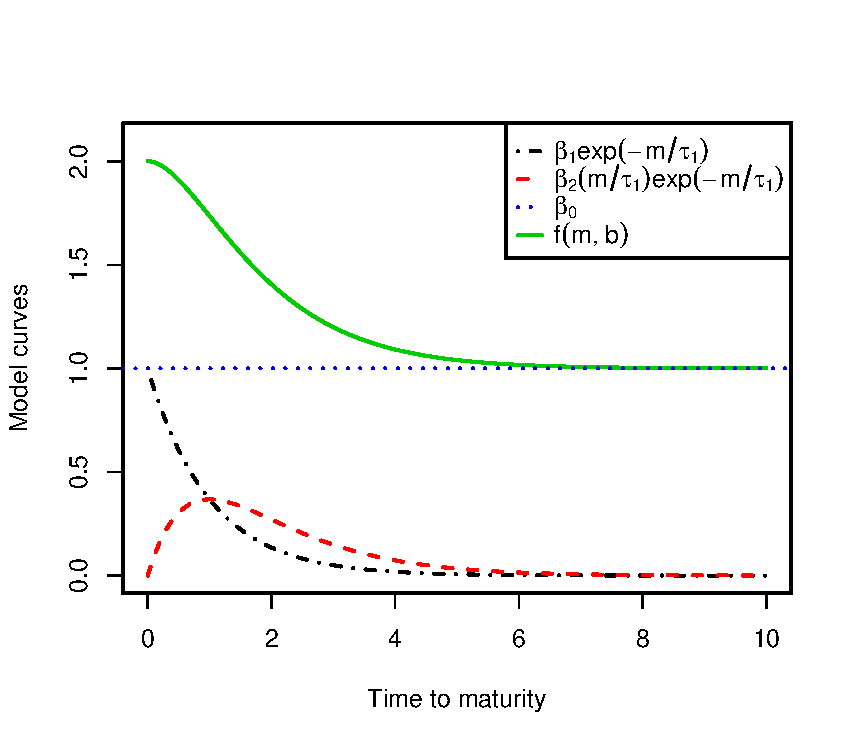
\includegraphics[width=0.7\textwidth]{pics/ns.pdf}
	\caption{to name}
\end{figure}


\cite{Svensson1994} extended the functional form by two additional parameters which allows for a second hump-shape. 

The spot rate is calculated as


\begin{multline}\label{sv_spot}
    s(m,\bm{b}) = \beta_0 + \beta_1\frac{1-\exp(-\frac{m}{\tau_1})}{\frac{m}{\tau_1}} + \beta_2\left(\frac{1-\exp(-\frac{m}{\tau_1})}{\frac{m}{\tau_1}} - \exp(-\frac{m}{\tau_1})\right) \\+ \beta_3\left(\frac{1-\exp(-\frac{m}{\tau_2})}{\frac{m}{\tau_2}} - \exp(-\frac{m}{\tau_2})\right), 
\end{multline}

with a parameter vector ${\bm{b}} = \left(\beta_0,\beta_1,\beta_2,\tau_1,\beta_3,\tau_2\right)$.

The impact of the paramteres can be described as follows \citep[cp.][p.7]{Bolder1999}:


\begin{itemize}
\item $\beta_0$ is the asymptotic value of the forward rate function.  The curve will tend torwards the asymptote as the time do maturity approches  $\infty$ ($\beta_0 >0$).
\item $\beta_1$ determines the starting (short-term) value of the curve in terms of deviation from the asymptote (the sum $\beta_0$ and $\beta_1$ is the vertical intercept. Morover, it defines the basic speed with wich the curve tends torward its long-term trend.
\item $\tau_1$ specifies the position of the first hump or the U-shape on the curve ($\tau_1>0$).
\item $\beta_2$ determines the magnitude and direction of teh hump. If $\beta_2 >0$  a hump will occur at  $\tau_1$, whereas $\beta_2<0$, a U-shaped value will occur at $\tau_1$.
\item $\tau_2$ specifies the position of the second hump or the U-shape on the curve ($\tau_2>0$).
\item $\beta_3$ analogously  to  $\beta_2$ determines the magnitude and direction of the second hump.  
\end{itemize}

The following code replicates the figure 1 on page 8 in \cite{Bolder1999}. The figure shows the decomposition of the forward rate curve. 


\begin{figure}[h]
\centering
	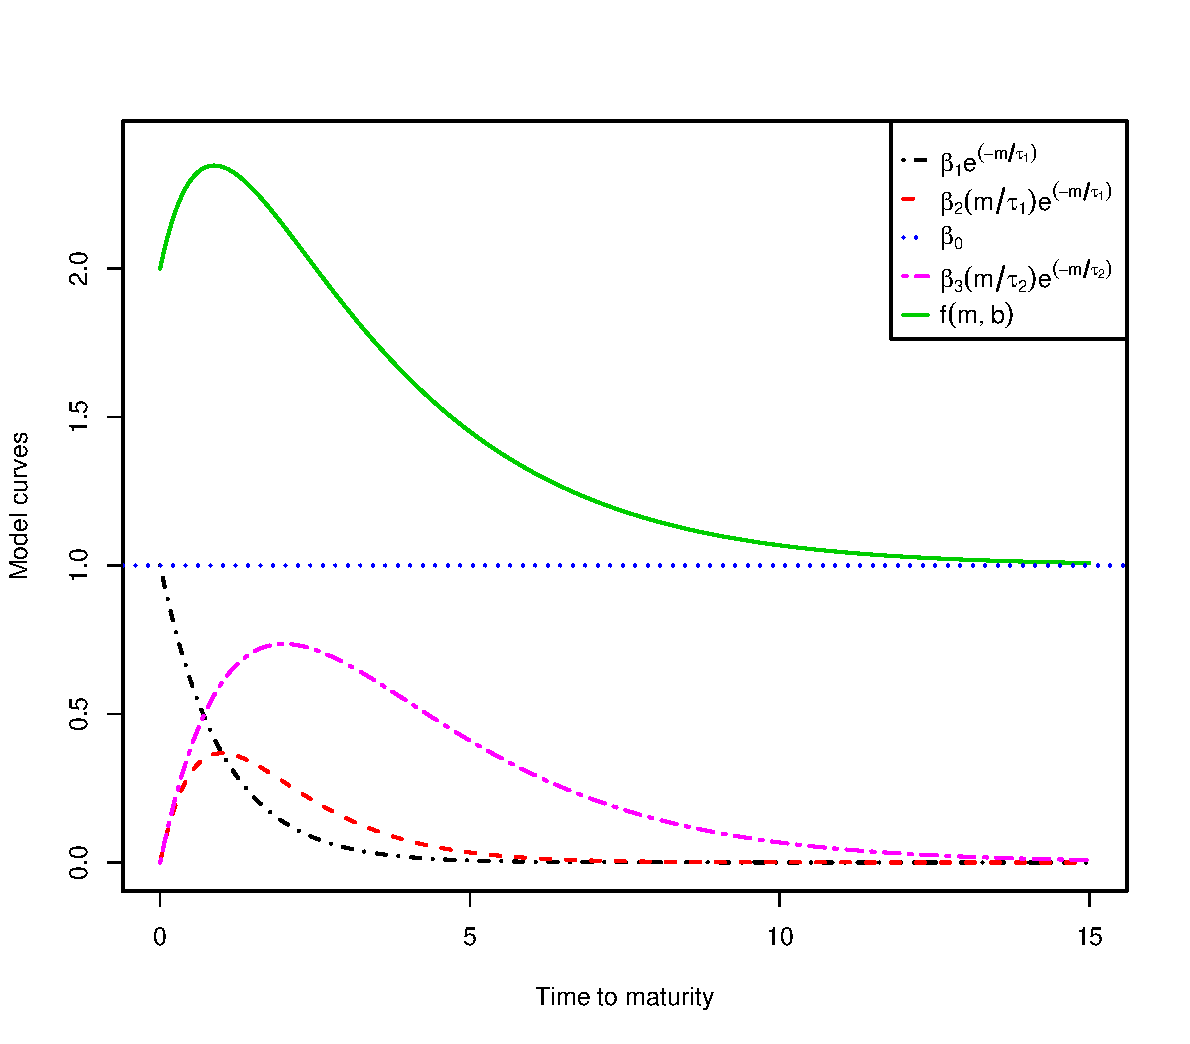
\includegraphics[width=0.7\textwidth]{pics/sv.pdf}
	\caption{to name}
\end{figure}

\begin{verbatim}

m <- seq(0,15,0.01)
beta_1 <- 1
tau_1 <- 1
beta_2 <- 1
beta_0 <- 1
tau_2 <-2
beta_3 <- 2


par(lwd=2)

#beta_1
plot(m,beta_1*exp(-m/tau_1),type="l",col=1,
     xlab="Time to maturity",
     ylab="Model curves",ylim=c(0,2.4),lty=4)
     
#beta_2     
lines(m,beta_2*(m/tau_1)*exp(-m/tau_1),lty=2,col=2)

#beta_3
lines(m,beta_3*(m/tau_2)*exp(-m/tau_2),lty=6,col=6)

#f
lines(m,beta_0+beta_1*exp(-m/tau_1)+beta_2*(m/tau_1)*exp(-m/tau_1) +
beta_3*(m/tau_2)*exp(-m/tau_2),col=3)

#beta_0
abline(h=1,lty=3,col=4)

legend("topright",legend=c(expression(beta[1]*e^(-m/tau[1])), 
       expression(beta[2]*(m/tau[1])*e^(-m/tau[1])),
       expression(beta[0]),
       expression(beta[3]*(m/tau[2])*e^(-m/tau[2])),
       expression(f(m,b))),
       lty=c(4,2,3,6,1), col=c(1,2,4,6,3))
\end{verbatim}


\subsection*{Credit-spread estimation}
The credit-spread estimation in the package termstrc is limited to the usual way for calculating a credit spread curve, i.e
 substracting the yield-curve of a reference country $s_{ref}(\mathbf{m,b})$ from the yield-curves $s_j(\mathbf{m.b})$ of other countries . 
 
 
\begin{equation}
cs_j(\mathbf{m}) = s_j(\mathbf{m,b}) - s_{ref}(\mathbf{m,b})
\end{equation}

\begin{tabular}{ll}
$cs_j(\mathbf{m})$ & credit-spread between country $j$ and reference country $ref$ \\
$s_j(\mathbf{m.b})$ &spot-rate curve of country $j$ with maturity vector  $\mathbf{m}$ \\
$s_{ref}(\mathbf{m,b})$ & spot-rate curve of the reference country 
\end{tabular}

Whereas the spot-rate functions are definied according to (\ref{ns_spot}),(\ref{sv_spot}) respectively. 
For a more advanced method of credit-spread calculation we refer to \citep{Jankowitsch2004}.

 \section{Estimation procedure}

The objective is to construct zero-coupon yield curves based on observable data of coupon bonds. As  explained above, a theoretical bond price can be estimated using the basic bond characteristics, which are quoted at the market. Therefore the challange of the optimisation is to minimize the deviation of the theoretical from the dirty price. The following explainations provide an insight in how the estimation problem may be structured. Moreover, we attach importance to an easy translation of the theoretical problem to a practical implemenation. Thus we use a matrix notation to explain the estimation procedure for an approach that estimates the yield curves for one group of bonds, e.g. country, rating class. 

\subsection{Construction of the basic matrices and vectors:}

\subsubsection*{Maturity Matrix $\bm{M}$: }

\begin{equation}\label{maturitym}
\bm{M}_{\left[n\times m\right]} = \{m_{ij}\}
\end{equation}

The number of rows $n$ is determined through the number of cashflows of the bond $j$ with the longest maturity. For each bond $j$ exists a column with the corresponding cashflowdates. Dates after the maturity of the bond $j$ are filled up with zeros till the maturity date of the bond with the longest maturity. One element $m_{ij}$ of the matrix  refers, therefore, to the maturity date of  the $i$-th cashflow of the $j$-th bond.

\subsubsection*{Cashflow Matrix $\bm{C}$:}
 
 \begin{equation}\label{cashflowm}
\bm{C}_{\left[n\times m\right]} = \{c_{ij}\}
\end{equation}
 
 The cashlflow matrix is defined analogously to the maturity matrix.  One element $c_{ij}$  of the matrix refers to the cashflow of the $i$-th cashflow of the $j$-th bond. Note, that the last cashflow of a bond $j$ also includes the redemption payment. 

\subsubsection*{Discount factor Matrix $\bm{D}$:}
  
 \begin{equation}\label{discountm}
\bm{D}_{\left[n\times m\right]} = \{d_{ij}\}
\end{equation}
 
 The discount factor matrix is defined analogously to the maturity matrix. One element $d_{ij}$ of the matrix refers to the discount factor associated with  the $i$-th cashflow of the $j$-th bond. One discount factor $d_{ij}$ is constructed as follows:
 
\begin{displaymath} 
d_{ij}=e^{-m_{ij}s(m_{ij},b)}
\end{displaymath}

Whereas $s(m_{ij},b)$ is the spot rate function defined in equation \ref{ns_spot}, \ref{sv_spot} according to Nelson/Siegel and Svensson, respectively. 

\subsubsection*{Clean price vector $\bm{p}^c$:}
 
  \begin{equation}\label{pc}
\bm{p}^c_{\left[1\times m\right]} = \{p^c_j\}
\end{equation}

$p_{c_j}$ is the quoted price of the j-th bond ($j=1...m$).

\subsubsection*{Accrued Interest vector $\bm{a}$: }

  \begin{equation}\label{a}
\bm{a}_{\left[1\times m\right]} = \{a_j\}
\end{equation}

There exists different conventions for the calculation of accrued interest. A basic form for the $j$-th bond is as follows.

\begin{equation}
    a_j= \frac{\mbox{number of days since last coupon payment}}{\mbox{number of days in current coupon period}}\cdot \mbox{coupon}_j
\end{equation}
 	


\subsubsection*{Dirty price vector $\bm{p}^d$:}

  \begin{equation}\label{pd}
\bm{p}^d_{\left[1\times m\right]}= \{p^d_j\}
\end{equation}
The dirty price vector is the sum of the clean price vector and the accrued interest vector and consists of the dirty prices of all bonds $j$.

\begin{displaymath}
\bm{p}^d=\bm{p}^c+\bm{a}
\end{displaymath}

\subsubsection*{Weights vector $\bm{w}$:}

  \begin{equation}\label{weights}
\bm{w}_{\left[1\times m\right]}= \{w_j\}
\end{equation}

Whereas $\omega_j$ is the weight for bond $j$ with Duration $d_j$:

\begin{displaymath}
w_j=\frac{\frac{1}{d_j}}{\sum_{i=1}^m\frac{1}{d_i}}
\end{displaymath}


The duration for a bond $j$ is a weighted average of the time to cashflows. 
%old definition
%\begin{equation}
  %\label{duration}
 % D=\frac{C\sum_{i=1}^n\delta(m_i)m_i+\delta(m_n)Rm_n}{C\sum_{i=1}^n\delta(m_i)+\delta(m_n)R}=\frac{1}{p_c+a}\left[C\sum_{i=1}^n\delta(m_i)m_i+\delta(m_n)Rm_n\right]
%\end{equation}

\begin{equation}\label{duration}
d_j= \frac{\bm{C}_{\left[n \times j\right]} \left(\bm{D}_{\left[n\times j\right]} \cdot \bm{M}_{\left[n\times j\right]}\right)^t} {\bm{C}_{\left[n \times j\right]}\left(\bm{D}_{\left[n\times j\right]}\right)^t}
\end{equation}

Whereas $(\cdot)$ denotes a element by element multiplication and $( )^t$ the transposed matrix (vector). 

%\subsubsection*{Fair bond prices $\bm{p}^f$}
%m�sste eine matrix sein 
%\begin{equation}
  %\label{eq:fairprices}
  %\bm{p}^f_{\left[1\times m\right]}=(\bm{C\cdot D})
%\end{equation}
%evtl. Def. Duration


\subsection{Formulation of the objective function:}
The objective functions aims at the minimisation of the sum of the weighted pricing errors. We focus on the minimization of pricing errors rather than YTM errors because yield calculations are more  time consuming. 
The specification of weights for the pricing errors avoids heteroscedasticity. The weights are determined according to equation \ref{weights} \citep{Bolder1999}


\subsubsection*{The objective function and the constraints}


\begin{equation}\label{constraints}
    \bm{b}_{opt} = \min_{b}\left(\left(\bm{\iota}_{\left[1 \times n\right]}\left[\bm{C}\cdot\bm{D}\right] - \bm{p}^d\right)^2 \bm{w}\bm{\iota}_{\left[m \times 1\right]} \right)
\end{equation} 

% \begin{equation}\label{constraints}
%     \bm{b}_{opt} = \min_{b}\left(\left(\bm{\iota}_{\left[1 \times n\right]}\left[\bm{C}_{\left[n \times m\right]}\cdot\bm{D}_{\left[n\times m\right]}\right] - \bm{p}^d_{\left[1\times m\right]}\right)^2 \bm{w}_{\left[1\times m\right]}  \bm{\iota}_{\left[m \times 1\right]} \right)
% \end{equation} 
 
The element by element multiplication of the cashflow matrix $\bm{C}$ with the discount factor matrix $\bm{D}$ returns a matrix with the present values of all cash flows. Multiplying this with a unit vector $\bm{\iota}$ from the left results in the vector of fair bond prices.  

 Whereas the vector $\iota$ contains only ones an the parameter vector is subject to constraints 
( $\beta_0 >0, \tau_1>0, \tau_2 > 0$). Using the optimal parameter vector  $\bm{b}_{opt}$ and the disired spot-rate function, the spot-rates can be calculated for a specified maturity vector $\bm{m}$. 
 
 \subsection{Specials consideration concerning the numerical optimisation}

The selection of the a good start parameter set is vital for an accurate numerical optimisation. \cite{Bolder1999} point out that the estimation difficulites derive from the 
spot rate function (forward rate function), which is linear in the betas , however, non-linear in the taus. Morover, there appear to multiple local minima in addition to the 
global minium. Therefore, in order to obtain a global minimum, a good start parameter set is required. 

 \cite{Bolder1999} present two different approaches for the generation of start parameters. The first one is based on an enumerationalgorithm. A Matrix with many different start parametersets is generated. For each set the optimization is performed and the best solution is chosen as the start parameter set for the final optimisation. 
The second approach divides the parameters into the linear an non-linear parameters. For the optimisation one group is held constant, whereas the other group is varied. This method improves the speed of convergence. 
 
 \cite{ferenczi2005} proposed an optimisation algorithm which is based on the HCP Algorithm of \cite{novak1996} and can be used for a start parameter algorithm. The advantage of this algorithm is, that it convergences  to the global minimum of the objective function. 

 \section{Examples}
 In this section we present the package in more detail. We describe the included data sets, the offered functions, methods and finally we conclude the section with a presentation of demo examples. 
 
 \subsection{Data sets}
 
 The package termstr includes two data sets in a list format. The first one (\verb|eurobonds|) consits of austrian, german, italian and hungarien government bond data. The second one (\verb|corpbonds| includes data of bonds from different rating categories (AAA,AA+,AA,AA-,A+,A,A-,BBB+,BBB,BBB-). For each bond the ISIN-code, maturity date, start date, coupon rate, price, accrued interest, cashflows, cashflow dates and the date stamp for the quoted price are required. 
The structure of the packages can be explored using the function \verb|str|:

\begin{verbatim}

List of 4
 $ AUSTRIA:List of 8
  ..$ ISIN        : chr [1:14] "AT0000383690" "AT0000383864" ...
  ..$ MATURITYDATE:Class 'Date'  num [1:14] 13614 21014 13893 ...
  ..$ STARTDATE   :Class 'Date'  num [1:14]  9962 10057 10241 ...
  ..$ COUPONRATE  : num [1:14] 0.0575 0.0625 0.0500 0.0413 0.0400 ...
  ..$ PRICE       : num [1:14] 104 135 105 105 104 ...
  ..$ ACCRUED     : num [1:14] 3.48 2.16 4.21 3.47 1.38 ...
  ..$ CASHFLOWS   :List of 3
  .. ..$ ISIN: chr [1:115] "AT0000383690" "AT0000383690"  ...
  .. ..$ CF  : num [1:115]   5.75 105.75   6.28   6.23   6.24 ...
  .. ..$ DATE:Class 'Date'  num [1:115] 13249 13614 13346 13710 ...
  ..$ TODAY       :Class 'Date'  num 13102
 $ GERMANY:List of 8
  ..$ ISIN        : chr [1:29] "DE0001134468" "DE0001134922" ...
  ..$ MATURITYDATE:Class 'Date'  num [1:29] 16972 19726 13517...
  ..$ STARTDATE   :Class 'Date'  num [1:29]  6014  8769  9865  9976 10046 ...
  ..$ COUPONRATE  : num [1:29] 0.0600 0.0625 0.0600 0.0600 0.0650 ...
  ..$ PRICE       : num [1:29] 121 132 104 105 139 ...
  ..$ ACCRUED     : num [1:29] 2.48 5.45 5.23 2.25 2.44 ...
  ..$ CASHFLOWS   :List of 3
....
....
....
\end{verbatim}
 
 
 \subsection{Functionality of the package}
 The complete functionality of the package is provided by the function \verb|termstrc_estim|, that is designed as follows:
 
\begin{verbatim}
termstrc_estim(countries, bonddata, maturity_spectrum, method, fit,
                           weights, startparam,control)
\end{verbatim}

whereas the parameters have the following options and denotation:

\begin{table}[h]

\begin{center}
	\begin{tabular}{r  l l}	
		 parameter&denotation&e.g. \\	
		\hline
		\verb|countries|&countries vector &\verb|c("AUSTRIA", "ITALY")| \\ 
		\verb|bonddata|&data set&\verb|eurobonds|\\
		\verb|maturity_spectrum|&maturity spectrum &\verb|"all"| or e.g. \verb|c(1,20)|\\
		\verb|method|&Nelson/Siegel or Svensson&\verb|"Nelson/Siegel" od. "Svensson"|\\
		\verb|fit|&Opimization mehtod&\verb|"prices"| or  \verb|"yields"| \\
		\verb|weights|&Durationweighting&\verb|"none"| or \verb|"duration"|\\
		\verb|startparam|&start parameter vector& \verb|b<- matrix(rep(1,8),nrow=2)|\\
		\verb|control|&control parameter for \verb|nlminb|&\verb|control=list(eval.max=1000)|\\
	\end{tabular}
\end{center}
\caption{Denotation of the parameters of the function termstrc\_estim}
\end{table}

The first element of the \verb|countries| vector is used as the reference country for the credit-spread calculation. A specific 
start parameter algorithm has not been implemented. Therefore, a start parameter set for each country has to be provided by the user. 
The start parameter matrix for the countries Austria, Germany and Italy may look like this:


\begin{verbatim}
 	        beta0       beta1       beta2	      tau1
GERMANY 0.02547394 -0.01216259 -0.02547394    1
AUSTRIA 0.02611532 -0.01136742 -0.02611532    1
ITALY   0.02578871 -0.01520725 -0.02578871    1
\end{verbatim}

The function \verb|termstrc_estim| elements und sub-lists of the returned list are shown in table \ref{returnlist}.You may use this code to explore the structure of the returned list:

\begin{verbatim}
library(termstrc)
demo(euro01)
str(myres)
\end{verbatim}



\begin{table}[t]\label{returnlist}
	\begin{tabular}{r  l l}	
		 list element&content \\	
		\hline	
  \verb|maturity_spectrum| & Includes the chosen maturity spectrum\\		
  \verb|method| & Includes the chosen estimation method \\
  \verb|fit|&Includes the chosen objective function\\
  \verb|weights|&Includes the type of optimisation, i.e "none" or "duration" \\
  \verb|n_countries|&the number of countries (rating categories) used for the optimisation\\
  \verb|cashflows|&the cashflow matrix for all specified countries (sub-list)\\
  \verb|maturities|&the maturity matrix for all specified countries (sub-list)\\
  \verb|dirty_prices|&the dirty prices for all specified countries(sub-list)\\
  \verb|estimated_prices| &the estimated prices for all specified countries (sub-list)\\
  \verb|yields| & the calculated yields for all bonds of the specified countries (sub-list)\\
  \verb|opt_result|&the optimal parameter vector for the specified countries (sub-list)\\
  \verb|spotrates|&the spotrates calculated with the optimal parameter vector (sub-list)\\
	\end{tabular}
	
	\caption{content of the returned list of the function termstrc\_estim}
\end{table}


 
 \subsubsection*{S 3 Methods}

The package uses the \verb|R - S3| class definition. For the class \verb|termstrc_singlecurve| exists a \verb|summary|, \verb|print| and \verb|plot| method.  

The \verb|summary| method prints goodness of fit test for the price and yielddeviation (root mean square error and average absolute error) and convergence information of the used optimiser (\verb|nlminb|).
The \verb|print| method prints the optimal parameter set for the specified countries or rating categories. 
Different plots for the zero-coupon- yield curves  of the countries  and spread curves is provided by the \verb|plot| method. 


 \subsection{Demos}
 
 In this section we present a step by step guidance on how to use the package to estimate the term-structure. We use the included data sets. 

 
 \textit{Step 1:} Load the package and the desired data set
 
 \begin{verbatim}
 library(termstrc)
 data(eurobonds)
\end{verbatim}
 
 \textit{Step 2:} Set the parameters of the function \verb|termstrc| as required
 
 \begin{verbatim}
countries <- c("GERMANY", "AUSTRIA", "ITALY")
bonddata <- eurobonds
maturity_spectrum <- "all"
method = "Nelson/Siegel"
fit = "prices"
weights = "duration"
control=list(eval.max=100000)
b<-matrix(c(0.02547394, -0.012162592, -0.02547394,    1,
 			0.02611532, -0.011367422, -0.02611532,    1,
			0.02578871, -0.015207250, -0.02578871,    1),
			nrow=3,ncol=4,byrow=TRUE)
			
rownames(b)<-countries

colnames(b)<-c("beta0","beta1","beta2","tau1")

 \end{verbatim}
 
\textit{Step 3:} Assign the function  
  
  \begin{verbatim}
  myres<- termstrc_estim(countries, bonddata, maturity_spectrum, 
    method, fit, weights, startparam=b,control) 
\end{verbatim}

\textit{Step 4:} Use the S3 print method to get the optimised parameter set

\begin{verbatim}  
print(myres)
\end{verbatim}

\textit{Step 5:} Use the S3 summary method to get the goodness of fit test and the convergence info

\begin{verbatim}  
summary(myres)
\end{verbatim}

\textit{Step 6:} Use the S3 plot method to generate different plots of the termstructure and the spread-curves. By default the zero-coupon-yield curve is plotted separately for each specified country and for all countries together. Morover the spread-curves are plotted. 

\begin{verbatim}  
plot(myres)
\end{verbatim}

\begin{figure}[h]
\centering
	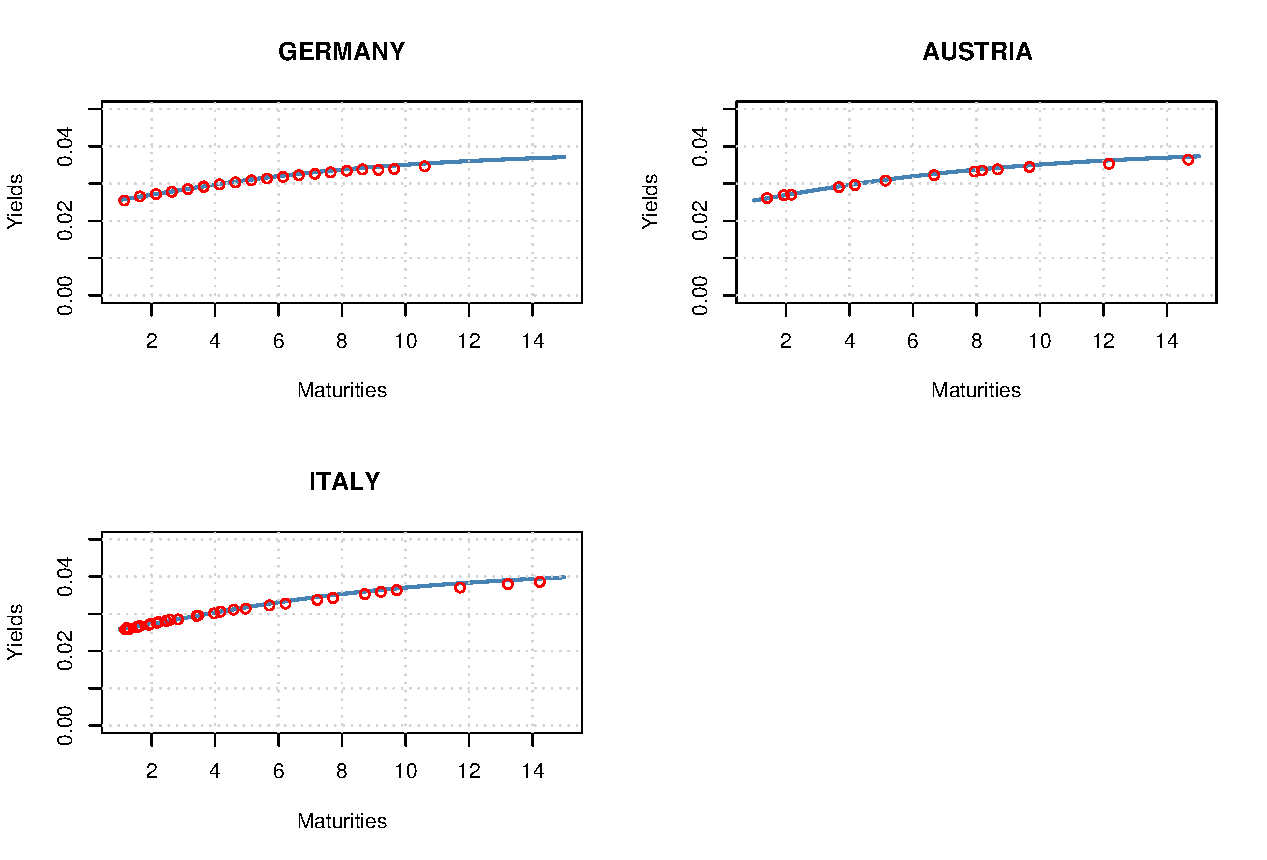
\includegraphics[width=0.8\textwidth]{pics/euro_nsg1.pdf}
	\caption{to name}
\end{figure}

\begin{figure}[h]
\centering
	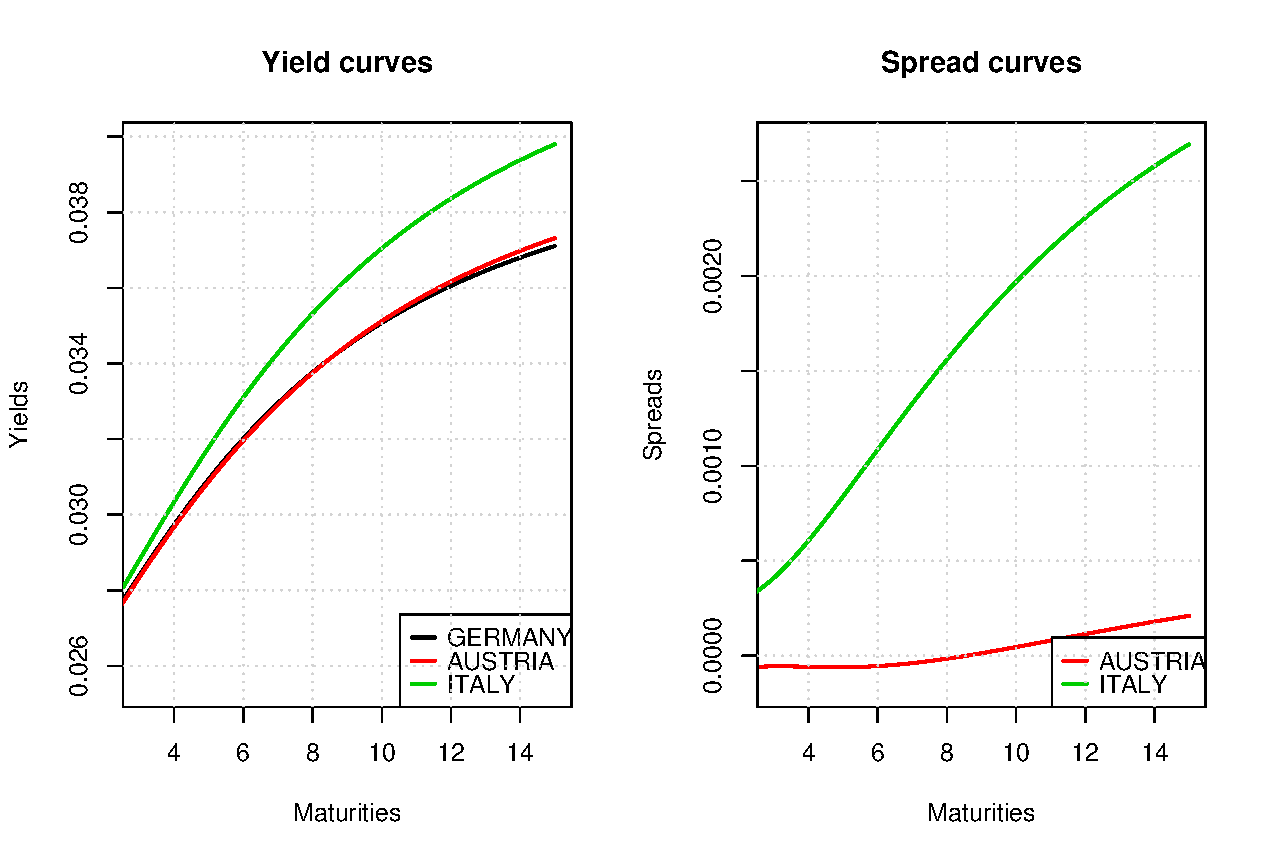
\includegraphics[width=0.8\textwidth]{pics/euro_nsg2.pdf}
	\caption{to name}
\end{figure}

The presented example is easily accessable using the demo function in R. Use \newline 
 \verb|demo(package="termstrc")| to explore the included demo examples. 


 
  \newpage 
 \section{Discussion}
 \newpage
 \section*{Acknowledgements}

  
 The authors are grateful to the students of the finance management science lab class of 2005.
 
 \section{TODO}
 
 \begin{itemize}
 \item Plot Methode (Fensteranpassung etc...)
 \item Code bereinigen/checken
 \item Funktionalit�t erweitern ( Zero Cupon bonds, Forwardrates)
 \item evtl neuer Datensatz
 \item Doku und Vignette �berarbeiten
 \end{itemize}
 

%\nocite{*}
\listoftables
\listoffigures
\bibliographystyle{unsrtnat}
\bibliography{termstrc}

  
  \end{document}